\cotefile{161-6}
\scanpage{2}
\mspage{\textcircled{6}}
\unsure{group|groupe|Groupes}

(Notes sur formes \unsure{paraboliques|paradoxiques} prêtées à \unsure{Labache|Laborde|Labarde|Lobarde|Loborde})

% margin note written sideways
\margin{Graphes, icosaèdre}
% archive sheet number: 1
\scanpage{4}
\uline{L'icosaèdre}

$E$ espace vectoriel euclidien de dim $3$\inserted{[espace vectoriel muni d'une forme quadratique non dégénérée, qu'on supposera définie positive au besoin]}, produit scalaire $x.y$ ($\|x\|=\sqrt{x^2}$).

$S$ la sphère unité $=\{x\in E\mid\|x\|^2=1\}$.

Si $u\in S$, $u^\perp$ désigne le plan orthogonal ; donc $u+u^\perp$ est le plan tangent à $S$ en $u$, tandis que l'espace vectoriel tangent à $u$ en $S$ est can. isom. à $u^\perp$

L'ensemble des directions tangentes en $u$ \deleted{sur} \inserted{à} la sphère \inserted{$S$} \unsure{s'identifie|s'identifient} à l'ensemble $u^\perp\cap S=\Sigma_u$ des vecteurs unité orthogonaux à $u$.

On suppose $E$ orienté, de sorte que \deleted{\unsure{à}} à un couple $u\in S,v\in\Sigma_u$ est associé un troisième vecteur $w=u\wedge v$, caractérisé par les conditions $w\in S\cap u^\perp\cap v^\perp$, $(u,v,w)$ orienté en sens direct.
\inserted{On peut dire que le plan $u^\perp$ est orienté : \deleted{\unsure{puisque|précisément}} la rotation d'angle $\frac{\pi}{2}$ $v\mapsto u\wedge v$ y est définie}

Le groupe spécial orthogonal $SO(E)$ opère de façon simplement transitive sur l'ensemble des directions tangentes à la sphère $S$ en ses différents points, i.e. l'ensemble des couples $(u,v)\in S$ avec $u.v=0$ i.e. $v\in\Sigma_u$. Le groupe orthogonal $O(E)\simeq\deleted{\text{\unsure{produit}}}SO(E).\deleted{\unsure{Z}}\unsure{\mu_2|\boldsymbol{\mu}_2}$ ($\mu_2={}$homothéties $\pm1$) opère de façon doublement transitive.

\deleted{\unsure{Soit les|Soit des}} \inserted{Les} points sur $S$ du grand cercle passant par $u$ dans la direction $v$, \deleted{sont} i.e. de $w^\perp\cap S$, sont de la forme
\[
x(u,v;\alpha)=u\cos\alpha+v\sin\alpha \qquad \alpha\ \text{défini mod }2\pi\mathbb Z
\]

D'autre part, les \deleted{\unsure{vecteurs|autres}} directions tangentes à $S$ en $u$, i.e. les \deleted{\unsure{k}} points de $u^\perp\cap S$, s'écrivent
\[
v'=v\cos\theta+w\sin\theta
\]

Fixons $\theta$, et calculons les carrés des côtés du triangle de sommets $u,x(u,v;\alpha),x(u,v',\alpha)$. On a

\figure{\begin{tikzpicture}[x=1cm,y=1cm,>=Stealth,scale=.86]
\coordinate (o) at (1.45,.95); \coordinate (u) at (1.95,2.65);
\coordinate (x) at (.46,3.38); \coordinate (y) at (.42,2.04);
\coordinate (v) at (.27,1.45); \coordinate (p) at (-.10,.70); \coordinate (w) at (.18,-.04);
\draw[->,thick] (o)--(u) node[right] {$u$};
\draw[->] (o)--(v) node[left] {$v$}; \draw (o)--(p) node[left] {$v'$};
\draw[->,thick] (o)--(w) node[below] {$w$};
\draw (v) to[bend right=27] (p) to[bend right=17] (w);
\draw[dashed] (o)--(x) (o)--(y);
\draw (x) node[above] {$x(u,v;\alpha)$} to[bend left=14] (u) to[bend right=13] (y) node[left] {$x(u,v';\alpha)$};
\draw (.75,.82) to[bend left=23] (.80,1.23) node[pos=.45,right] {$\theta$};
\draw (1.1,1.45) to[bend left=18] (1.62,1.52) node[pos=.53,above] {$\alpha$};
\draw (1.19,1.52) to[bend left=17] (1.60,1.61);
\draw (1.56,2.48) to[bend left=12] (1.60,2.92) node[pos=.55,left] {$\theta$};
\end{tikzpicture}}

\[
\resizebox{\linewidth}{!}{$\displaystyle
\left\{\begin{aligned}
\|x(u,v;\alpha)-u\|^2 &\underset{\substack{\text{par raison}\\\text{de sym.}}}{=}
\|x(u,v',\alpha)-u\|^2=(\cos\alpha-1)^2+\sin^2\alpha=2(1-\cos\alpha)=4\sin^2\frac{\alpha}{2}\\
\|x(u,v,\alpha)-x(u,v',\alpha)\|^2&=\sin^2\alpha\,\|v-v'\|^2=\sin^2\alpha\,4\sin^2\frac{\theta}{2}
=\left(4\sin^2\frac{\alpha}{2}\cos^2\frac{\alpha}{2}\right)\left(4\sin^2\frac{\theta}{2}\right)
\end{aligned}\right.$}
\]
% archive sheet number: 3
\scanpage{5}
Donc pour que ces trois points forment un triangle équilatéral (il est de toutes façons \unsure{isoscèle|isocèle}) il fst que l'on ait
\[
\deleted{\unsure{4}}\cos\frac{\alpha}{2}=\pm\frac{1}{2\sin\theta/2}\quad\deleted{\unsure{\sin}}\ .\tag*{\textcircled{1}}
\]
\margin{[\uline{NB} Un tel $\alpha$ existe sss $|\sin\frac{\theta}{2}|\geq\frac12$, i.e. si $0\leq\theta\leq\pi$, sss \inserted{sss} $\frac{\pi}{6}\leq\frac{\theta}{2}\leq\frac{5\pi}{6}$ i.e. $\deleted{\unsure{\pi/3|\frac{\pi}{3}\leq}}\boxed{\theta\geq\frac{\pi}{3}}$]}
ou encore, comme $\cos\alpha=\cos^2\frac{\alpha}{2}-\sin^2\frac{\alpha}{2}=2\cos^2\frac{\alpha}{2}-1$
\[
\cos\alpha=\frac{1}{2\sin^2\theta/2}-1=\deleted{\unsure{\cos\theta}}\frac{1-2\sin^2\theta/2}{2\sin^2\theta/2}
=\frac{\cos\deleted{\unsure{2}}\theta}{2\sin^2\theta/2}=\frac{\cos\theta}{1-\cos\theta}\tag*{\textcircled{$1'$}}
\]
% slanted
\margin{\uline{NB} $\left\{\begin{aligned}\cos2\alpha&=-\frac35\\\cos\alpha&=\frac{1}{\sqrt5}\end{aligned}\right.$ pour $\theta=\frac{2\pi}{5}$}

Bien entendu, dans ce cas, les autres ``angles dièdres'' définis par ce triangle en les deux autres sommets, sont également égaux à $\theta$. On a en fait construit ici, \inserted{choisissant la détermination principale de $\alpha$ comme $0<\alpha<\pi$,} \uline{le} seul triangle équilatéral inscrit dans la sphère $S$, d'angle dièdre $\theta$, ayant un sommet en $u$, un \deleted{\unsure{côté|autre}} \inserted{deuxième sommet $x$} dans la direction tangente $v$ à $S$ en $u$, et \deleted{situé} tel qu'avec le troisième sommet $x'$ l'orientation $u,x,x'$ soit directe.

Nous allons fixer par la suite
\[
\theta=\frac{2\pi}{5}\tag*{\textcircled{2}}
\]
et, pour quelque temps, on fixe $u$ et $v$. On posera
\[
v_i=v\cos i\theta+w\sin i\theta\qquad i\in\mathbb Z/5\mathbb Z\tag*{(3)}
\]
(de sorte que $v_0=v$, i.e. $v_i=v$ si $i\equiv0\ (5)$), et on posera
\[
\deleted{\unsure{v_i=v\ \text{si }i\equiv0\ (5)}}
\]
\[
\begin{aligned}
x_i&=x(u,v_i,\alpha)=u\cos\alpha+v_i\sin\alpha
% Both occurrences of sin alpha carry a transposition stroke to before the preceding factor.
=u\cos\alpha+v\sin\alpha\cos i\theta+w\sin\alpha\sin i\theta\\
&& (i\in\mathbb Z/5\mathbb Z)
\end{aligned}\tag*{(4)}
\]
\margin{\uline{NB} Il est immédiat que les $u,x_i$ sont $6$ pts \uline{distincts} (leurs projections sur le plan $u^\perp$ sont $0$ et les $v_i\sin\alpha$) à coordonnée suivant $u>0$ ; donc les $u,u'$, $x_i',x_i$ sont $12$ points \uline{distincts} de $S$}

où $\alpha$ est fixé par (1) ou (1$'$), $0<\alpha<\pi$. On trouve donc cinq points en ordre circulaire sur le cercle de \inserted{centre $u$} rayon (rectiligne) $4\sin^2\frac{\alpha}{2}$ tracé sur la sphère $S$. On pose de plus
\[
x'_i=-x_i,\quad u'=-u\qquad (i\in\mathbb Z/5\mathbb Z)\tag*{(5)}
\]
\margin{On appelle cet ens de 12 pts l'\uline{icosaèdre} défini \uline{par} $u,v$.}

Un ensemble de points $(x,y,z)$ de $S$ \inserted{définissant un triangle équilatéral} d'angle au centre $\alpha$ est appelé un \uline{triangle icosaèdral} ; \inserted{cela signifie aussi qu'il y a une rotation qui l'amène en $(u,x_0,x_1)$} un ensemble de points $(a,b_0,b_1,\ldots,b_4)$ \inserted{de $S$} est appelé un \uline{calotte d'icosaèdre} s'il existe une transformation \inserted{orthogonale} $g\in O(E)$ qui l'amène en l'ensemble précédent $(u,x_0,x_1,\ldots,x_4)$ ; Il revient encore au même \deleted{que} de dire \inserted{son cardinal est $6$, et que l'on peut ordonner cet ens. de telle façon que} que les triangles $(a,b_i,b_{i+1})$ pour $0\leq i\leq3$ sont icosaèdraux (et alors $(a,b_4,b_0)$ est aussi icosaèdral$^{*}$. Le point $a$ est alors uniquement
% archive sheet number: 4
\scanpage{6}
\margin{$*$ Ou encore que les longueurs des dix vecteurs $a-b_i$ ($0\leq i\leq4$), $b_i-b_{i+1}$ ($0\leq i\leq4$, posant $b_5=b$) sont égales à
\(\ell=2\sin\frac{\alpha}{2}\) \textcircled{4}. Notons les longueurs correspondantes des vecteurs $a-b'_i=a+b_i$ \textcircled{$4'$} $\ell'=2\cos\frac{\alpha}{2}$}
% slanted
\margin{Notons que $\ell^2$ et $\ell'^2$ sont les solutions de l'équation quadratique $\lambda^2-4\lambda+4\sin^2\alpha=0$}

déterminé, \deleted{et l'ens} on l'appelle le \uline{sommet} de la calotte d'icosaèdre, \inserted{les autres points les \uline{points périphériques} ;} \deleted{et} Sur l'ensemble des \deleted{\unsure{directions}} \inserted{ceux-ci} (grâce à l'orientation \inserted{de $E$ donc} de $S$, \deleted{\unsure{donne|donc}} il y a alors un ordre circulaire canonique, qui en fait un torseur sous le groupe $\mathbb Z/5\mathbb Z$. Le sous-groupe \inserted{$G_C$} de $G=O(E)$ qui laisse une calotte $C$ invariante, \deleted{\illegible{1}} a dix éléments, \deleted{le sous-g} son intersection \inserted{$G'_C$} avec $G'=SO(E)$ est le groupe (can. isom. à $\mathbb Z/5\mathbb Z$) des rotations d'angle multiple de $2\pi/5=\theta$ autour du \deleted{\unsure{sommet}} \inserted{vecteur} $a$. \deleted{On obtient un} \inserted{Les cinq} points de $G_C\cap\complement G'_C$ sont \inserted{d'ordre 2, et forment avec l'élément neutre} les stabilisateurs dans $G_C$ des cinq points périphériques de la calotte ; l'élément $g_i\in G_C\cap\unsure{\complement G'_C|\complement C'_C}$ qui laisse $b_i$ invariant est la symétrie p.r. au plan engendré par $a,b_i$. La structure du groupe $G_C$ est le produit $1/2$ direct du \deleted{\unsure{\mathbb Z/5\mathbb Z}} sous-groupe $G_C$ (can. isom à $\mathbb Z/5\mathbb Z\inserted{{}=\mu_5}$) et du groupe $\mathbb Z/2\mathbb Z$, opérant sur $G_C$ par symétrie. Enfin, le groupe $G'_C\simeq\mathbb Z/5\mathbb Z=\mu_5$ opère de façon simplement transitive sur l'ens des pts périphériques de la calotte (ce qui redonne une définition de \deleted{leur} l'ordre circulaire can. sur leur ens.)

Jusqu'à maintenant le choix $\theta=2\pi/5$ n'a pas joué de rôle particulier : on aurait pu prendre $\theta=2\pi/m$, et le groupe des $m$ rotations multiples de $2\pi/m$ aurait rempli un rôle analogue. Cela va changer avec le

\uline{Lemme} L'ensemble $(x_0;x_1,u,x_{-1},x'_2,x'_{-2})$ est une calotte d'icosaèdre de sommet $u$, l'ordre circulaire canonique étant celui écrit

\uline{Démonstration} Faisant la symétrie p.r. au plan engendré par $u,x_0$ (qui échange $x_1$ et $x_{-1}$, $x'_2$ et $x'_{-2}$) on est ramené \inserted{(à une question d'orientation près)} à montrer que les \deleted{trois triangles} longueurs des trois vecteurs $x_0-x'_2,\ x_{-1}-x'_2,\ x'_2-x'_{-2}$ sont égales à la (4) -- et on on peut se dispenser de la \inserted{vérifier pour} dernier vecteur. \deleted{\unsure{De même on a}} Il sera plus astucieux de montrer que si on \deleted{\unsure{a}} \inserted{considère} l'élément \inserted{$\gamma^w_\alpha$} de $G'=SO(E)$ qui est \deleted{l'identité sur $w$, et qui dans le plan $(u,v)$ est} la rotation d'angle $\alpha$ autour de $w$ et l'élément $\gamma^u_{-\frac{\theta}{2}}$ qui est la \deleted{identité sur $u$ et qui est} \inserted{rotation} d'angle $-\theta/2$ autour de $u$, et si on pose
% archive sheet number: 5
\scanpage{7}
\inserted{$\gamma=\gamma^w_\alpha\gamma^u_{-\theta/2}$, alors} transforme la calotte $(u,(x_i)_{i\in\mathbb Z/5\mathbb Z})$ en l'\deleted{calotte} \inserted{ensemble} dit, plus précisément que l'on a les six relations
\[
\gamma u=x_0,\quad\deleted{\unsure{x}}\gamma x_0=x'_{2},\quad\gamma x_1=x'_{-2},\quad\gamma x_2=x_1,\quad\gamma x_3=u,\quad\gamma x_4=x_{-1}
\]

Faisons le calcul :
\[
\resizebox{\linewidth}{!}{$\displaystyle\begin{aligned}
\gamma u&=\gamma^w_\alpha\deleted{\unsure{=}}(u)=u\cos\alpha+v\sin\alpha\\
\gamma v&=\gamma^w_\alpha(v\cos\tfrac{\theta}{2}-w\sin\tfrac{\theta}{2})=(-u\sin\alpha+v\cos\alpha)\cos\tfrac{\theta}{2}-w\sin\tfrac{\theta}{2}\\
&=-u\sin\alpha\cos\tfrac{\theta}{2}+v\cos\alpha\cos\tfrac{\theta}{2}-w\sin\tfrac{\theta}{2}\\
\gamma w&=\gamma^w_\alpha(+v\sin\tfrac{\theta}{2}+w\cos\tfrac{\theta}{2})=(-u\sin\alpha+v\cos\alpha)\deleted{\unsure{(}}\sin\tfrac{\theta}{2}\deleted{\unsure{)}}+w\cos\tfrac{\theta}{2}\\
&=-u\sin\alpha\sin\tfrac{\theta}{2}+v\cos\alpha\sin\tfrac{\theta}{2}+w\cos\tfrac{\theta}{2}
\end{aligned}$}
\]
\[
\gamma=\begin{pmatrix}
\cos\alpha&-\sin\alpha\cos\frac{\theta}{2}&-\sin\alpha\sin\frac{\theta}{2}\\
\sin\alpha&\cos\alpha\cos\frac{\theta}{2}&\cos\alpha\sin\frac{\theta}{2}\\
0&-\sin\frac{\theta}{2}&\cos\frac{\theta}{2}
\end{pmatrix}
\]
\[
\begin{aligned}
\gamma u&=u\cos\alpha+v\sin\alpha=x_0\qquad\text{OK}\\
\gamma x_0&=\gamma u\cos\alpha+\gamma v\sin\alpha
=u(\cos^2\alpha-\sin^2\alpha\cos\tfrac{\theta}{2})+v(\sin\alpha\cos\alpha+\sin\alpha\cos\alpha\cos\tfrac{\theta}{2})\\
&\hspace{9em}-w(\sin\alpha\sin\tfrac{\theta}{2})
\end{aligned}
\]
Or $x'_2=-x_2=-u\cos\alpha-\deleted{\unsure{\frac{1}{4}}}v\sin\alpha\cos2\theta-w\sin\alpha\sin2\theta$ % transpose marks on both pairs of factors

à prouver
\[
\left\{\begin{aligned}
-\cos\alpha&=\cos^2\alpha-\sin^2\alpha\cos\tfrac{\theta}{2}\\
-\cos2\theta\deleted{\sin\alpha}&=\deleted{\sin\alpha}\cos\alpha(1+\cos\tfrac{\unsure{\theta}}2)\\
\deleted{\unsure{w}}\deleted{\sin\alpha}\sin2\theta&=\deleted{\sin\alpha}\sin\tfrac{\theta}{2}
\end{aligned}\right.
\]
\[
\begin{aligned}
\gamma x_1&=\gamma u\cos\alpha+\gamma v\sin\unsure{\alpha|\theta}\cos\theta+w\sin\alpha\sin\theta\\
&=
\end{aligned}
\]
% archive sheet number: 6
\scanpage{8}
\uline{Cor.} Soit \deleted{\unsure{que}} $g\in G=O(E)$ transformant la calotte $(u,(x_i))$ en celle du lemme. Alors $g$ invarie l'icosaèdre $I=I_{uv}$

En effet, il est immédiat que l'icosaèdre associé à cette \inserted{deuxième} calotte est encore $I$.

Soit $\Gamma_I\inserted{{}=\Gamma_{u,v}}$ le sous-groupe de $G=O(E)$ qui laisse l'icosaèdre \inserted{$I=I_{u,v}$} invariant, $\Gamma'=\Gamma\cap G'$ le sous-groupe formé des rotations de $\Gamma$. Il est clair que $\Gamma'$ est d'indice 2 dans $\Gamma$ (N.B. $-1\deleted{\unsure{\notin}}\in\Gamma\cap\complement\Gamma'$) et que $\Gamma$ est d'où la produit
\[
\Gamma\simeq\mu_2\times\Gamma'
\]

\uline{Théorème} $\Gamma'$ opère de façon transitive sur l'ens. des sommets de l'icosaèdre, $I$, et de façon simplement transitive sur l'ens des couples $(x,\deleted{\unsure{y}}d)$ où $x$ est un sommet de l'icosaèdre, $I$ une arrête. $\Gamma$ opère de façon \inserted{simplement} transitive sur l'ens des triples $(x,y,z)$ de points de $I$ formant une face$^{*}$
% slanted
\margin{$*$ On peut aussi bien sur l'ens des triples d'arrêtes formant une face -- c'est évidemment équivalent}

On a oublié de préciser que par définition les \uline{arrêtes} de l'icosaèdre $I$ sont les \inserted{30} segments \deleted{de longueur $\ell$ qui joignent :} \inserted{suivants}
\[
\left\{\begin{aligned}
(u,x_i),&\qquad \deleted{\unsure{x_{i+1}}}(u',x'_i)\\
(x_i,x_{i+1}),&\qquad (x'_i,x'_{i+1})\\
(x_i,x'_{i-2})&\qquad (x'_i,x_{i-2})
\end{aligned}\right.\qquad i\in\mathbb Z/5\mathbb Z
\]
% slanted
\margin{Ce sont aussi les \unsure{ensembles} à deux éléments \inserted{distincts} $(x,y)$ de l'icosaèdre, de distance minimum (laquelle est $\ell$) -- sera plus facile à vérifier après transitivité de $\Gamma'$ sur l'ens des sommets}

De plus, on appelle \uline{faces} de l'icosaèdre une \deleted{partie} \inserted{des 20 \deleted{\unsure{ensembles}} parties} de $3$ \deleted{\unsure{éléments}} \inserted{trois} éléments \deleted{qui fait partie des \inserted{20} ensembles} suivants (ou les triangles qu'ils déterminent)
\[
\begin{aligned}
(u,x_i,x_{i+1})&\qquad (u',x'_i,x'_{i+1})\\
(x_i,x'_{i-2},\underset{\substack{\Vert\\x_{i+1}}}{x_{i\unsure{-}4}})&\qquad
(x'_i,x_{i-\unsure{1|2}},\underset{\substack{\Vert\\x'_{i+1}}}{x'_{i-4}})
\end{aligned}\qquad i\in\mathbb Z/5\mathbb Z
\]
% slanted
\margin{Ce sont aussi les triples \inserted{$(x,y,z)$} tels que $(x,y)$ $(y,z)$ et $(z,x)$ soient des arrêtes. Il y en a exactement \uline{cinq} issus de \deleted{sommet} \inserted{contenant} $u$ comme sommet. Ici aussi, ce sera immédiat à vérifier \uline{après} la transitivité.}

\uline{Démonstration} On sait déjà que les points $x_i$ \deleted{\unsure{sont situés}} sont congruents sous $\Gamma'$, et par symétrie les points $x'_i=-x_i$ aussi. De plus le lemme nous montre que $u$ est congruent à $x_0$, \deleted{$x_0$ est congru} (donc par symétrie $u'$ l'est à $x'_0$), et \deleted{par} $x_0$ \unsure{à} $x'_2$ -- donc tous les $x_i$ sont congruents. \deleted{Pour montrer} \inserted{Montrons} que $\Gamma'$ est \inserted{simplement} transitif sur l'ens des couples $(x,d)$ i.e des arrêtes \uline{orientées} $(x,y)$, \deleted{\unsure{il}} i.e que si $(x',y')$ en est une autre alors $\exists!\ g\in\Gamma'$, $gx'=x,gy'=y$. On peut supposer $x=u,y=x_0$, et par la transitivité déjà établie sur les sommets, $x'=u$. Donc \deleted{\unsure{en vertu comme}} \inserted{alors} $y'$ est un des $x_i$, \deleted{\unsure{et l'on sait}} \inserted{Il est clair} que le stabilisat\unsure{eur}
% archive sheet number: 7
\scanpage{9}
% slanted
\margin{\deleted{\unsure{que}} Précisons que tout point de l'icosaèdre est centre d'une \deleted{\unsure{déterminée}} unique calotte d'icosaèdre contenue dans $I$ ; la calotte de centre $a$ est formée de $a$ et de tous les pts \uline{reliés} à $a$ par une arrête. \deleted{\unsure{Elle est}} \deleted{\unsure{unique}}}
\margin{Données équivalentes :
$\left\{\begin{array}{l}
\text{icosaèdre + un des sommets}\\
\text{icosaèdre + calotte d'icosaèdre contenue dedans}\\
\text{calotte d'icosaèdre}\\
\text{une couple }(u,v)\text{ modulo rotation sur }v\\
\quad\text{dans }u^\perp\text{ d'angle multiple de }\theta
\end{array}\right.$
[point du fibré principal sur $S$ de groupe $\mathbb T$ \unsure{de|,} puissance cinquième du fibré fourni \unsure{des|du} \unsure{$(u,v)$|$u,v$}, \unsure{soit|\ldots}}

de $u$ dans \deleted{\unsure{G}} $\Gamma'$ est aussi le sous-groupe \deleted{de} $G'$ \deleted{formé des} des $g\in G'$ qui invarient la calotte $(u,(x_i))$, lequel, nous avons vu, est le groupe $\mu_5$ qui opère de façon simplement transitive sur l'ens des $x_i$, OK.

Prouvons enfin l'assertion de \inserted{simple} transitivité de $\Gamma$ sur l'ens. des \deleted{faces} triples $(x,y,z)$ qui sont de face. Procédant comme dessus, on peut supposer, utilisant ce qui est déjà démontré, que $x=x'=u,y=y'=x_0,z=x_1$. Mais il n'y a que deux \deleted{triangles} faces \deleted{\unsure{en}} admettant $(u,x_0)$ comme arrête, leurs autre sommet est resp. $x_1$ et $x_{-1}$. Si c'est $x_{-1}$, la symétrie p.r. au plan $u,v$ (qui évidemment invarie l'icosaèdre $I$) transforme $x_{-1}$ en $x_1$ en laissant $u,x_0$. Il reste donc : \deleted{vérifier} noter que $u,x_0,x_1$ \deleted{\unsure{x_{-1}}} étant linéairement indépendants une transformation linéaire qui fixe ces trois points est l'identité.

\uline{Corollaire} $\Gamma'$ est d'ordre 60, $\Gamma$ d'ordre 120.

Le premier point provient du fait que l'icosaèdre a 30 arrêtes, donc $2.30=60$ arrêtes orientées. Comme $\Gamma\simeq\Gamma'\times\mu_2$, on trouve que $\Gamma$ a 120 éléments. On peut aussi noter qu'il y a 20 faces, chacune ayant \deleted{\unsure{deux|trois}} six ordres totaux sur l'ens de ses sommets, ce qui fait $6\times20=120$ triples ordonnés faisant face.

\uline{Remarque} Les sommets et arrêtes de l'icosaèdre forment (avec leur relation d'incidence) un \uline{graphe}, et $\Gamma'$ opère par automorphismes de ce graphe. Montrons que \uline{tout} automorphisme \inserted{$g$} du graphe est dans $\Gamma'$. On est ramené à \deleted{\unsure{en}} prouver \deleted{\unsure{pour}} qu'un autom. du graphe qui fixe $u,x_0,x_1$ \deleted{\unsure{g}} est l'identité. Prouvons qu'il est l'identité sur tous ces points $x_i$ (\inserted{i.e. tous les pts de $I$,} qui peuvent être reliés à \unsure{l'un|un} des sommets -- $u$ en l'occurrence -- par une arrête) : en effet \deleted{\unsure{on}} pour $x_0,x_1$ il n'y a rien à prouver, or $x_2$ ($x_{-1}$) est l'unique point de $I$ \inserted{distinct de $x_0$ (resp. $x_1$)} qui est relié \deleted{par} à la fois à $u$ et $x_1$ ($u$ et $x_0$), donc il est fixé, donc aussi $x_3$ (p. ex. comme
% archive sheet number: 8
\scanpage{10}
l'unique autre point de $I$, à part $x_{-1},x_0,x_1,x_2$, qui sont reliés à $u$). Donc \deleted{\unsure{l'ens|l'un}} \inserted{chacun} des points \deleted{fixes} de la calotte standard \deleted{\unsure{est}} de centre $u$ est fixe. La $=$ chose est vrai pour les points de la calotte de centre $x_0$, donc aussi [appliquant \unsure{ceci|ces} aux triangles $(u,x_i,x_{i+1})$) à ceux \deleted{\unsure{la}} calottes \unsure{de|du} centre $x_i$, $i\in\mathbb Z/5\mathbb Z$. Mais Cela donne \uline{tous} les points \inserted{de $I$} sauf $u'$, or celui-ci doit être fixe aussi comme le complémentaire du \unsure{V|v|l'} ens précédent !

\deleted{Ainsi, on} On peut aussi regarder l'ens des faces et l'ens des arrêtes de l'icosaèdre $I$ \inserted{et leur relation d'incidence} (NB une arrête est déterminée par l'ens. des deux faces qui la contiennent), ils forment encore un graphe (dont les ``sommets'' sont les ``faces de l'icosaèdre ; \deleted{\unsure{en fait|on}} \inserted{ce} serait le graphe des sommets-arrêtes du dodécaèdre, \uline{dual} à l'icosaèdre). Je dis que le groupe des automorphismes de ce graphe est encore $\unsure{\Gamma|\Gamma'}$ [NB il est \deleted{immédiat} \inserted{évident} que $\Gamma$ y opère de façon fidèle]. On est encore ramené \unsure{à} prouver que tout autom. de ce graphe qui \deleted{\unsure{laisse}} invarie une face donnée et ses trois arrêtes, disons \deleted{\unsure{u,x_0,x_1}} encore $(u,x_0,x_1)$, est l'identité. Or il invarie alors chacun des \inserted{trois} triangles adjacents (comme les uniques triangles adjacents distincts sur les trois arrêtes envisagées), \deleted{et \unsure{on sait|invarie} alors leurs arrêtes (?)} puis les \deleted{triangles} faces $(u,x_2,x_3)$ et $(u,x_3,x_4)$ comme les seul couple de faces adjacent mutuellement, \uline{et} adjacents resp. à $(u,x_1,x_2)$ et $(u,x_0,x_{-1})$ (dont on sait qu'ils sont invariants). Cela donne l'invariance des \deleted{\unsure{les faces des deux}} arrêtes $(u,x_2)$ et $(u,x_4)$ commes intersection, donc aussi des arrêtes restantes $(x_1,x_2)$ et $(x_0,x_{-1})$ des deux \deleted{triangles} faces $(u,x_1,x_2),(u,x_0,x_{-1})$. Donc leurs arrêtes sont fixes, \deleted{\unsure{\illegible{2}|donc}} et par symétrie on voit que pour chacune des \deleted{triangles} \inserted{faces} adjacentes à $(u,x_0,x_1)$, \deleted{les \unsure{trois}} ces faces \uline{et} leurs arrêtes sont fixes. À partir de là la conclusion est triviale
% archive sheet number: 9
\scanpage{11}
On voit ainsi que les propriétés des actions de $\Gamma,\deleted{\unsure{\Gamma'}}$ sur les ens de sommets, arrêtes et faces de l'icosaèdre (\deleted{ensembles} munis de leurs relations d'incidence mutuelles) sont conséquences de la seule structure combinatoire de ces ensembles (soit \deleted{Il convient} sommets-arrêtes, soit faces-arrêtes, soit \unsure{mieux|même} le triple système sommets-arrêtes-faces \ldots). Il convient cependant de caractériser le sous-groupe $\Gamma'$ de $\Gamma$ en termes combinatoires, On peut dire p. ex. que c'est le groupe qui respecte \inserted{les} ordres circulaires qu'on a sur les \inserted{ens. des points périphériques des} calottes \deleted{sphériques} de \deleted{\unsure{l'icosa}} l'icosaèdre (en termes de la structure combinatoire, on peut définir \uline{deux} ``syst. cohérents'' d'ordres circulaires sur les calottes \deleted{\unsure{sphér}} $\inserted{\unsure{\pm}}$, correspondants aux deux orientations possibles de l'espace ambiant).
% archive sheet number: 10
\scanpage{13}
% archive sheet number: 12
\[
\unsure{\zeta|\xi}^3+\zeta^{-1}+\zeta+\zeta^{-3}=\zeta+\zeta^2+\zeta^3+\zeta^4=-1
\]
L'équation de $\gamma$ est donc
\[
\boxed{\gamma^2+\gamma-1=0}
\]
donc
\[
\unsure{\mathbb V_5|\mathcal V_5|\mathfrak D_5|\vartheta_5}=\mathbb Z[\tfrac15][t]/(t^2+t-1)
\]
\[
\boxed{\gamma=(-1\pm\sqrt5)/2}
\]
\margin{\deleted{si 2 inv.} Cette formule garde un sens sur tt schéma où $2$ \uline{et} $5$ sont inversibles}

\[
\begin{aligned}
2\cos\frac{2\pi}{5}&=(\sqrt5-1)/2\\
\cos\frac{2\pi}{5}&=\frac{\sqrt5-1}{4}\\
\cos\frac{4\pi}{5}&=\frac{-\sqrt5-1}{4}
\end{aligned}
\qquad
\begin{aligned}
(2\gamma+1)^2&=5\\
\deleted{\unsure{4\gamma^2+4\gamma=4}}&\\
\unsure{e|c}^2+e-1&
\end{aligned}
\]
\[
\begin{aligned}
&(-1+\sqrt5)/2\\
&=\bigl((-1-\sqrt5)/2\bigr)^2-2=\\
&\qquad\frac{1+5+2\sqrt5}{4}-2=\deleted{\unsure{4}}-\tfrac12+\tfrac12\sqrt5
\end{aligned}
\]
\[
\begin{aligned}
\zeta&\mapsto\zeta^2\\
\zeta&\unsure{\mapsto|\vdash}\zeta^3
\end{aligned}
\qquad\text{si }\zeta+\zeta^{-1}=t
\]
\figure{\begin{tikzpicture}[scale=.88,>=Stealth]
\draw (.35,1.48) .. controls (1.22,1.94) and (2.55,1.45) .. (2.53,.28)
.. controls (2.48,-.92) and (1.91,-1.62) .. (.92,-1.53)
.. controls (.07,-1.50) and (-.36,-1.20) .. (-.41,-.66);
\draw (-.41,.96) --(-.16,.64) (.05,.48)--(.85,.03)--(1.50,1.57);
\draw (-.42,.03)--(.85,.03)--(1.56,-1.23);
\draw[->] (.85,.03)--(2.51,.10);
\draw[->,thick] (.85,.03)--(-.45,-.84);
\draw (.85,.03)--(-.38,-.69);
\draw (2.48,-.12) .. controls (2.42,-.66) and (2.35,-.94) .. (2.02,-1.03);
\end{tikzpicture}}
\[
\deleted{\unsure{\cos^{\ell}\ D,x,D|\cos' D,D}}
\]
\[
\cos^{\unsure{\ell|1|\prime}}_{\unsure{q|4}}(D,\unsure{\zeta}D)=\operatorname{Tr}\zeta^2=\zeta^2+\zeta^{-2}=\underline{t^2-2}
\]
\[
\begin{aligned}
t',t''\qquad t''&=t^{\prime 2}-2=(t^{\prime\prime 2}-2)^2-2\\
t'&=t^{\prime\prime 2}-2
\end{aligned}
\]
\diagram{$\begin{array}{cccc}
\zeta&\zeta^2&\zeta^3&\zeta^4\\
&&\Vert&\Vert\\
&&\zeta^{-2}&\zeta^{-1}
\end{array}$}
\diagram{$\begin{array}{cccc}
\zeta+\zeta^{-1}&\zeta^2+\zeta^{-2}&\zeta^3+\zeta^{-3}&\zeta^4+\zeta^{-4}\\
\Vert&\Vert&\Vert&\Vert\\
\unsure{y|\gamma|\eta}=y_1&y_2&y_2&\zeta_1
\end{array}$}

% lower edge, written upside down; the implication arrow crosses the final column above
\[
\begin{aligned}
\text{d)}\quad\gamma((\unsure{V|\mathcal V}_\lambda))\leq\alpha_\lambda(V'_\lambda)
&\Longrightarrow V_\lambda\leq V'_\lambda\quad\text{\uline{ou}}\quad\exists\mu\ne\lambda\ \text{avec } V_\mu=0_{I_\mu}\\
\text{e)}\quad\gamma((V_\lambda))&\subset\operatorname{Sup}_i W_i\quad\Longrightarrow
\end{aligned}
\]
\scanpage{14}
% archive sheet number: 13
% Manuscript read after a half-turn. One long oblique stroke crosses the working.
\deleted{\[
\resizebox{\linewidth}{!}{$\displaystyle\begin{aligned}
&=\operatorname{Sup}\bigl[\bar\alpha(U)\cap\bar\beta(\unsure{V|W})\bigr]\cap
\bigl[\bar\alpha(U')\cap\bar\beta(V')\bigr]
=\bigl(\operatorname{Sup}\bar\alpha(U)\cap\bar\beta(V)\bigr)\cap
\bigl(\operatorname{Sup}\bar\alpha(U')\cap\bar\beta(V')\bigr)\\
&=\gamma(W)\cap\gamma(W')\qquad\text{OK}
\end{aligned}$}
\]
\unsure{$\gamma$)|c)} $\bar\gamma$ commute aux Sup quelconques
\[
\bar\gamma(\underbrace{\underset{\substack{\Vert\\\operatorname{Sup}}}{\operatorname{Sup}} W_i}_{W})\geq\operatorname{Sup}\bar\gamma(W_i)\quad\text{clair, prouvons }\leq
\]
\[
\operatorname{Sup}_{\gamma(U\times V)\subset\operatorname{Sup} W_i}\bar\alpha(U)\cap\bar\beta(V)
\qquad\text{à prouver que l'on a }\bar\alpha(U)\cap\bar\beta(V)\leq\operatorname{Sup}_i\bar\gamma(W_i)
\]
Or on aura, si $\gamma(U\times V)\subset\operatorname{Sup}W_i$
\[
\begin{aligned}U&=\operatorname{Sup} U_j\\V&=\operatorname{Sup} V_k\end{aligned}
\ \big|\ \forall j,k\quad\exists i\quad\text{avec }\gamma(U_j\times V_k)\leq W_i
\]
Donc
\[
\begin{aligned}
\bar\alpha(U)\cap\bar\beta(V)&=(\operatorname{Sup}_j\bar\alpha(U_j))\cap(\operatorname{Sup}_k\bar\beta(V_k))\\
&=\operatorname{Sup}_{j,k}\bar\alpha(U_j)\cap\bar\beta(\unsure{W_k|V_k})\qquad(\overset{?}{\leq}\operatorname{Sup}_i\bar\gamma(W_i))
\end{aligned}
\]
et comme \inserted{$\exists i/$} $\gamma(U_j\times V_k)\leq W_i$, on a
\[
\bar\alpha(U_j)\cap\bar\beta(W_k)\leq\bar\gamma(W_i)\leq\operatorname{Sup}_{i'}\bar\gamma(W_{i'})\qquad\text{cqfd}
\]

Généralisation aux sommes (produits) \unsure{infinies|infinis} :
\[
(I_\lambda)_{\lambda\in\Lambda}\qquad I_\lambda\in\operatorname{Ob}(\unsure{OM|CM})
\]
-- $\prod' I_\lambda$ : partie du produit formé des $(V_\lambda)$ tels que $V_\lambda=1_{I_\lambda}$ pour presque tt $\lambda$
\[
\alpha_\mu^0:I_\mu\longrightarrow\prod'_{\unsure{I|\lambda}} I_\lambda
\qquad\alpha_\mu^0(x)_\lambda=\begin{cases}x&\text{si }\lambda=\mu\\1_{I_\lambda}&\text{si }\lambda\ne\mu\end{cases}
\qquad\text{appl. cr.}
\]
\[
\begin{aligned}
\gamma &: \prod' I_\lambda\longrightarrow K &&\text{flèche dans }(OM)\\
\alpha_\mu&=\gamma\circ\alpha_\mu^0:I_\mu\longrightarrow K &&\text{appl. cr.}\qquad\text{On suppose}
\end{aligned}
\]
a) Les $\alpha_\mu$ commutent aux Sup quelc.

b) $\gamma$ commute aux Inf finis [en particulier
\[
\gamma((V_\lambda))=\mathop{\operatorname{Inf}}_\lambda\alpha_\lambda(V_\lambda)\qquad\text{(Inf en fait fini)}\ ;\ \text{et}
\]
les $\alpha_\mu$ sont des morphismes de $(OM)$]

c) Tout élément de $K$ est le sup d'éléments de $\prod'_\lambda I_\lambda$

TSVP}
\scanpage{15}
\[
\underset{\substack{\unsure{\wr\Vert|\Vert|\simeq}\\\mathbb Z/4\mathbb Z}}{\Gamma=(\mathbb Z/5\mathbb Z)^*}
\]
\diagram{\begin{tikzcd}[ampersand replacement=\&,column sep=small,row sep=small]
\mu_5 \arrow[d,dash] \& {\supset}\ \mu_5^* \arrow[d,dash]\& \deleted{\unsure{B}}\ \tau=\mu_5^*/\beta\\
\underset{\unsure{(\mathrm{id},d)|(0,d)|(\alpha,\alpha')}}{\operatorname{Spec}\mathbb Z} \arrow[r,phantom,"\unsure{\supset|\longrightarrow|\longleftarrow}" description] \& \mathbb Z[\tfrac15] \arrow[ur,dash] \&
\end{tikzcd}}
fini étale de \deleted{\unsure{degré}} rang 4 sur $\mathbb Z[\frac15]$ ; \deleted{\unsure{galoisien}} Galoisien de groupe $\Gamma$

engendré par $\unsure{\zeta|\xi}+\bar\zeta=\zeta+\zeta^{-1}=\unsure{\eta|\gamma}$
\inserted{$\zeta$\ $\rightarrow$ racine primitive universelle}

\margin{deux générateurs 2 et 3 \inserted{$=-2$} mod 5. un élément \inserted{$-1$} d'ordre 2 $-1$ ou 4 mod 5. un élément d'ordre 1 \quad 1 mod 5}
Sur $\mu_5(S)$ l'effet est $\zeta\mapsto\zeta^2$ ou $\zeta\mapsto\zeta^{-2}=\zeta^3$ resp.
\[
\begin{aligned}\zeta&\mapsto\zeta^{-1}=\zeta^4\\
\zeta&\mapsto\zeta\end{aligned}
\]
\diagram{\begin{tikzcd}[ampersand replacement=\&,row sep=small,column sep=1pt]
B\arrow[d,dash]\&{\supset B^\Gamma}\\ A\&
\end{tikzcd}}
\[
\left\{\begin{aligned}B&=A[\zeta]/\deleted{\unsure{T=}}\\
&A[T]/(1+T+T^2+T^3+T^4)
\end{aligned}\right.
\]
\[
T\mapsto T^4
\]
\figure{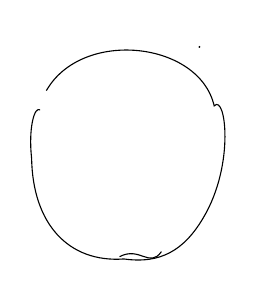
\begin{tikzpicture}[scale=.72]
\draw (.22,2.25) .. controls (.85,3.35) and (2.92,3.12) .. (3.18,1.98)
.. controls (3.38,2.20) and (3.55,.95) .. (2.99,.01)
.. controls (2.65,-.57) and (2.23,-.81) .. (1.59,-.72)
.. controls (.60,-.79) and (-.02,-.09) .. (-.04,1.05)
.. controls (-.10,1.59) and (.01,1.98) .. (.11,1.91);
\draw (1.51,-.68) .. controls (1.87,-.49) and (2.04,-.89) .. (2.25,-.59);
\fill (2.92,3.02) circle (.018);
\end{tikzpicture}}

\({}_nU\) étale de rang $n$ sur $\mathbb Z$ si on prend \deleted{\unsure{\({}_nU\)}} $\mu_n$ \uline{tordu} par $T$
\diagram{\begin{tikzcd}[ampersand replacement=\&,row sep=small,column sep=small]
\&\mu_n\arrow[d,phantom,"\cup"]\&\\
\varphi(n)\arrow[dr,dash]\arrow[r,dash]\&\mu_n^*\arrow[d]\&(\mathbb Z/n\mathbb Z)^*\\
\&S\&
\end{tikzcd}}
\[
\zeta\unsure{\mapsto|\vdash}\zeta^{-1}
\]
\[
\begin{aligned}
\beta(T)&=T^{-1}=T^4=-(1+T+T^2+T^3)\\
\beta(T^2)&=T^{-2}=T^3\\
\beta(T^3)&=T^{-3}=T^2\\
\beta(T^4)&-
\end{aligned}
\]
\[
1=T^0/T\quad T\quad T^2\quad T^3
\]
\diagram{\begin{tikzcd}[ampersand replacement=\&,row sep=small,column sep=small]
\text{gp}\&\mu_n^T\arrow[d,phantom,"\cup"]\&{\subset U}\\
\text{pas groupe}\&\mu_n^{*T}\arrow[d,"\substack{\text{étale}\\\text{rang }2}"']\&{\subset U}\arrow[d,"\operatorname{Tr}_{K/O}"]\&\zeta+\zeta\\
\&\mathbb V_n^T=V_n\arrow[d,"\substack{\text{étale}\\\text{rang }\varphi(n)/2}"']\&{\subset O}\\
\&S\&
\end{tikzcd}}
\[
\underset{\displaystyle\prod(p_i^{\alpha_i}-p_i^{\alpha_i-1})}{\underset{\Vert}{\varphi(n)}}\qquad
\begin{aligned}
\beta(c_0+c_1T+c_2T^2+c_3T^3)&\deleted{\unsure{=c_0+}}\\
&=c_0\unsure{+|-}c_1(-1+T+T^2+T^3)\\
&\qquad{}+c_2T^3+c_3T^2\\
&=(c_0-c_1)-c_1T+(c_3-c_1)T^2+(c_2-c_1)T^3\\
&\overset{?}{=}c_0+c_1T+c_2T^2+c_3T^3
\end{aligned}
\]
\[
(\mathbb Z/n\mathbb Z)^*\ni-1\qquad\mu_n\subset G_m
\]
\[
p^{n}-p^{n-1}=p^{n-1}(p-1)
\]
\diagram{\begin{tikzcd}[ampersand replacement=\&,row sep=small,column sep=small]
\mu_n^*\arrow[d] \& {\subset G_m}\arrow[d,"\unsure{\rho|c}"]\\
\mathbb V_n \& {\subset\mathbb E^1}
\end{tikzcd}}
\[
\rho(\lambda)=\lambda+\lambda^{-1}\qquad c_1=0\qquad c_2=c_3
\]
\[
\zeta+\zeta^{\deleted{\unsure{2}}-1}\ \bigg|\ \begin{aligned}\frac{p-1}{2}&=2\\ &\cos\end{aligned}
\qquad c_0+c_2(T^2+T^3)
\]
\[
\begin{aligned}
1+\zeta+\zeta^2+\zeta^3+\zeta^4&=0\\
\zeta+\zeta^{-1}&=\deleted{\unsure{\alpha}}\gamma
\end{aligned}
\qquad
\begin{aligned}
\operatorname{Tr}\gamma&=\gamma+\gamma^\sigma=\zeta+\zeta^{-1}+\zeta^2+\zeta^{-2}\\
&=\zeta+\zeta^2+\zeta^3+\zeta^4=-1\\
N\gamma&=\gamma\gamma^{\unsure{\sigma|\alpha}}=(\zeta+\zeta^{-1})(\zeta^2+\zeta^{-2})=
\end{aligned}
\]
% archive sheet number: 14
\scanpage{16}
Alors $\alpha,\beta$ :
\diagram{\begin{tikzcd}[ampersand replacement=\&,column sep=small,row sep=1pt]
I\arrow[dr]\&\\
\&K\\
J\arrow[ur]\&
\end{tikzcd}}
\inserted{sont dans $(\unsure{OM|CM})$ (grâce à a) b)) Je dis qu'ils} font de $K$ une somme de $I,J$ dans $(OM)$

% The long diagonal meets the body of the argument and stops above 2°.
\deleted{a) $\alpha,\beta$ épimorphiques i.e. pour $L\ \unsure{\in}\operatorname{Ob}(OM)$,
\[
\begin{aligned}
(*)\quad\operatorname{Hom}^{\unsure{\varphi}}_{OM}(K,L)&\longrightarrow\operatorname{Hom}_{OM}(I,L)\times\operatorname{Hom}_{OM}(J,L)\\
\varphi&\longmapsto(\varphi\circ\alpha,\varphi\circ\beta)
\end{aligned}
\]
injectif

En effet, si on connait $\varphi\circ\alpha$ et $\varphi\circ\beta$, i.e. $\varphi$ sur les $\unsure{\beta_*|\gamma_*|\gamma}(x\times1)$ et $\gamma_*(1\times y)$, on les connait sur leur $\cap$ donc sur $\gamma_*(x\times y)$ (par b)) donc sur les Sup de tels \unsure{pts|objets} de $\operatorname{Im}\gamma_*$, donc sur tout $K$ (par c).

b) $(*)$ est \unsure{surjectif|surjective}. Donnons-nous donc
\[
\bar\alpha:I\longrightarrow\unsure{L|K}\qquad\bar\beta:J\longrightarrow L\qquad\text{dans }(OM)
\]
définissons une application
\[
\bar\gamma:K\longrightarrow L
\]
par
\[
\bar\gamma(W]=\operatorname{Sup}_{\substack{U\in I\\V\in J\\\gamma(U\times V)\subset W}}\bar\alpha(U)\cap\bar\beta(\unsure{W|V})
\]
$1^\circ$) Prouvons d'abord
\[
\bar\gamma\circ\alpha=\bar\alpha,\quad\bar\gamma\circ\beta=\bar\beta
\]
Or
\[
(\bar\gamma\circ\alpha)(U')=\bar\gamma(U'\times1)=\operatorname{Sup}_{\gamma(U\times V)\leq\gamma(U'\times1)}
\bar\alpha(U)\cap\bar\beta(V)
\]
Or les $U\times V$ en question sont, en vertu de d), ceux pour lesquels ou bien $V=0_I$ (l'élémt correspondant du Sup est alors $\unsure{0_K}$, et ne compte pas) ou bien \deleted{ceux} pour lesquels $U\subset U'$, $V$ quel. donc le Sup est $\bar\alpha(U')\cap\bar\beta(1)=\bar\alpha(U')$ OK. On prouve de $=$ que $\bar\gamma\circ\beta=\bar\beta$}

$2^\circ$) Prouvons que $\bar\gamma$ est un morphisme de $(OM)$.

$\alpha$) $\bar\gamma$ croissant : clair

$\beta$) $\bar\gamma$ commute aux Inf finis.
\[
\bar\gamma(1_K)\deleted{\unsure{\overset{\mathrm{def}}{=}\bar\gamma(\gamma(1_I\times1_J))}}
\overset{\mathrm{def}}{=}\bar\alpha(1_I)\cap\bar\beta(1_J)=1_K
\]
\margin{Inf de famille vide}
\[
\resizebox{\linewidth}{!}{$\displaystyle
\bar\gamma(W\cap W')=\operatorname{Sup}_{\gamma(U\times V)\subset W\cap W'}\bar\alpha(U)\cap\bar\beta(W)
=\operatorname{Sup}_{\substack{\gamma(U\times V)\subset W\\\gamma(U'\times\unsure{V'|U'})\subset W'}}
\bar\alpha(U\cap U')\cap\bar\beta(V\cap V')$}
\]
\margin{[$\text{d'où }\gamma(U\cap U'\times V\cap V')\subset W\cap W'$ via b)}
% archive sheet number: 15
\scanpage{17}
\unsure{$K$|$k$}
\diagram{\begin{tikzcd}[ampersand replacement=\&,column sep=small,row sep=small]
\underline X\arrow[r]\&(\mathrm{Ens})\\
\underline{\hat X}\arrow[r,dash]\&(\mathrm{Ens})
\end{tikzcd}}
\unsure{contrairement|correspondant} aux \unsure{liens}
\margin{$9\times8$\qquad \unsure{Db|D5} \unsure{6} \unsure{689|789|989}}

\figure{\resizebox{\linewidth}{!}{\begin{tikzpicture}[x=.012cm,y=-.012cm,line cap=round,line join=round,>=Stealth]
% crop-candidate: scan 17
% The upper row, including the faint open shapes between the darker sketches.
\draw (285,176)--(365,101)--(409,185)--cycle (285,176)--(352,148)--(365,101) (352,148)--(409,185);
\draw (285,176) to[bend left=10] (382,162); \draw (326,125)--(332,131);
\draw[gray] (601,164) .. controls (648,121) and (712,149) .. (707,201) .. controls (705,238) and (656,267) .. (617,254) .. controls (597,245) and (579,194) .. (601,164);
\draw[gray] (613,250) .. controls (686,285) and (629,337) .. (574,338);
\draw[gray] (729,133) .. controls (677,48) and (758,21) .. (804,52) .. controls (852,81) and (810,131) .. (761,137);
\draw (760,137)--(771,73)--(813,103); \draw[gray] (863,55) .. controls (884,64) and (925,60) .. (940,79) .. controls (914,96) and (896,121) .. (916,140) (869,63)--(903,137);
\draw[->] (907,226)--(923,169);
\draw[->] (974,176)--(1036,176);
\draw[gray] (1051,197)--(1079,182) (1053,137)--(1051,197); \fill (1052,197) circle (2);
\draw[gray] (1075,166)--(1107,133)--(1146,166)--(1111,197)--cycle (1075,166)--(1146,166) (1107,133)--(1111,197);
\draw[gray] (1596,84) .. controls (1628,48) and (1699,72) .. (1670,133) .. controls (1657,166) and (1614,155) .. (1596,111) .. controls (1591,99) and (1590,91) .. (1596,84);
\draw[gray] (1635,148)--(1633,118)--(1668,95);
\draw[line width=1.3pt] (860,189) .. controls (813,172) and (756,217) .. (789,257) .. controls (814,285) and (852,255) .. (854,226);
\draw (784,238) to[bend right=9](854,222);
\draw[thick] (821,212)--(883,184)--(878,244)--cycle (821,212)--(855,214)--(883,184) (855,214)--(878,244);
\fill (739,208) ellipse (7 and 3); \draw (750,204)--(759,207);
% Small solid at the upper right with faint and dark edges.
\draw[gray] (1386,148)--(1433,73)--(1524,81)--(1484,157)--cycle (1386,148)--(1456,118)--(1524,81);
\draw[very thick] (1433,73)--(1415,266)--(1524,81)--cycle;
\draw[thick] (1415,266)--(1456,118)--(1524,81) (1415,266)--(1484,157);
\foreach \x/\y in {1386/148,1433/73,1524/81,1484/157,1456/118,1415/266}{\fill (\x,\y) circle (3);}
\draw (1384,137) circle (2) (1457,103) circle (3);
\end{tikzpicture}}}

$x<e$\qquad $x\quad y$\qquad $z\ \to\ x\cap y$
% margin note written sideways
\margin{Corolle}
\figure{\resizebox{\linewidth}{!}{\begin{tikzpicture}[x=.012cm,y=-.012cm,line cap=round,line join=round,>=Stealth]
% Crescent, corolla and stem, followed by the large three-petal sketch.
\draw (353,261) to[bend left=5] (488,196) .. controls (488,245) and (407,296) .. (353,261);
\draw (420,231)--(424,236);
\fill (248,342) circle (4); \draw[thick] (248,342) .. controls (279,387) and (310,431) .. (355,456);
\draw (222,447) .. controls (156,438) and (179,362) .. (221,357) .. controls (259,361) and (270,419) .. (250,439) --cycle;
\draw[thick] (222,447) .. controls (176,476) and (154,456) .. (156,426) .. controls (163,392) and (194,430) .. (222,447);
\draw (222,447) .. controls (284,402) and (317,444) .. (309,464) .. controls (291,486) and (246,460) .. (222,447);
\draw (222,447) .. controls (276,457) and (270,507) .. (224,518) .. controls (164,518) and (160,463) .. (207,449);
\draw (585,348)--(678,344)--(723,401) .. controls (691,439) and (635,473) .. (599,450) .. controls (573,437) and (567,394) .. (585,348);
\draw (679,336) .. controls (679,276) and (800,289) .. (827,307) .. controls (855,323) and (851,357) .. (855,381);
\draw (723,401)--(786,452) .. controls (798,467) and (846,446) .. (857,420);
\draw (723,401) .. controls (701,418) and (683,431) .. (663,454) --(664,516) .. controls (691,535) and (742,537) .. (775,528) .. controls (804,500) and (815,465) .. (787,451);
\fill (723,401) circle (5);
\draw[fill=black!45] (852,383) .. controls (906,368) and (909,453) .. (868,467) .. controls (808,485) and (775,400) .. (827,384) --cycle;
\begin{scope}\clip (846,423) ellipse (48 and 48);
\foreach \i in {0,...,24}{\draw[thin,gray] ({785+4*\i},371) .. controls ({826+3*\i},407) and ({791+3*\i},423) .. ({835+4*\i},475);}
\end{scope}
% Six sectors and the long returning arcs to G, X_0 and X_1.
\draw (970,306)--(1038,305)--(1074,364)--(1032,418)--(946,408)--(932,350)--cycle;
\draw (997,358)--(970,306) (997,358)--(1038,305) (997,358)--(1074,364) (997,358)--(1032,418) (997,358)--(946,408) (997,358)--(932,350);
\draw[very thick] (970,306)--(997,358)--(1045,306)--cycle;
\draw[very thick] (978,306)--(1027,306)--(1057,269)--(996,274) (972,307)--(1009,307)--(1046,271) (1073,271)--(1097,271);
\draw[->,thick] (997,358) .. controls (1053,320) and (1119,289) .. (1168,216) node[above] {$G$};
\draw[thick] (1117,287) .. controls (1139,346) and (1116,433) .. (1063,450) .. controls (1023,471) and (1005,456) .. (997,410);
\draw[thick] (938,364) .. controls (877,461) and (940,511) .. (1029,448);
\node at (1167,294) {$O(3)$}; \node at (1171,341) {$SO(3)$};
\draw[gray,->] (1120,345)--(1089,345);
\draw[->,very thick] (1129,448)--(1063,448); \node[right] at (1129,447) {$X_0$}; \node[below left] at (1063,445) {$X_1$};
\end{tikzpicture}}}

$\unsure{G}$ opère sur un \unsure{hom|hom.|homogène} $X\simeq G/H$ \unsure{univers} \unsure{tel} à [$\text{ex : }S^2$] et sur un $E$ (ens des parties de $S^2$).
\[
\operatorname{Hom}_G(X,E)\subset\operatorname{Hom}_{\unsure{G|C}}(P_{\unsure{s|S}},E)
\qquad \simeq E\deleted{\unsure{^G}}
\]
à savoir l'ens des flèches $g\mapsto gx$ telles que l'on ait $gx=ghx$ i.e. $E^H$

\diagram{\begin{tikzcd}[ampersand replacement=\&,column sep=large]
4\arrow[r]\&3\arrow[r]\&2\arrow[r,dash]\&1\arrow[r,dash]\&0
\end{tikzcd}}
\figure{\resizebox{\linewidth}{!}{\begin{tikzpicture}[x=.012cm,y=-.012cm,line cap=round,line join=round,>=Stealth]
% Pencil loops crossing the central row, folded quadrilaterals and isolated marks.
\draw[gray] (355,556) .. controls (330,491) and (403,415) .. (458,451) .. controls (489,476) and (513,556) .. (523,567) .. controls (477,623) and (378,628) .. (355,556);
\draw[gray] (430,448) .. controls (425,379) and (471,349) .. (523,395) .. controls (577,439) and (606,538) .. (552,561);
\draw[thick] (390,469) .. controls (418,477) and (446,489) .. (475,489);
\draw (465,538)--(566,527)--(596,594)--(521,600)--cycle;
\draw[thick] (565,527)--(521,601)--(519,673)--(594,596);
\draw[gray] (274,614) .. controls (287,591) and (315,631) .. (322,657) .. controls (294,645) and (280,632) .. (274,625);
\draw (335,685)--(387,662) (355,631)--(375,706);
% Flower beside the order and stalk labels.
\draw[gray] (940,575) .. controls (960,554) and (988,547) .. (1007,575) .. controls (1010,610) and (953,653) .. (939,618) .. controls (930,606) and (933,587) .. (940,575);
\draw (1007,575) .. controls (967,553) and (961,520) .. (987,496) --(1042,504)--(1045,557)--(1007,575);
\draw (1007,575) .. controls (1027,549) and (1060,559) .. (1086,575) --(1096,605) .. controls (1069,625) and (1037,625) .. (1020,607);
\draw (1007,575)--(982,617) .. controls (995,647) and (1020,657) .. (1045,637) --(1034,599)--cycle;
\fill (1007,575) circle (5); \draw[very thick] (1058,541)--(1134,501);
\node at (1126,552) {$y\leq x$};\node at (1142,607) {$O_x\subset O_y$};
% Nested neighbourhoods. The large outer curve reaches into the row below.
\draw (523,749) .. controls (345,768) and (481,657) .. (514,655) .. controls (642,608) and (816,597) .. (944,613) .. controls (1046,631) and (1040,717) .. (938,741) .. controls (797,759) and (634,760) .. (523,749);
\draw (620,658) .. controls (682,603) and (835,604) .. (922,626) .. controls (1009,649) and (985,696) .. (902,709) .. controls (772,726) and (640,706) .. (616,681) .. controls (610,674) and (612,667) .. (620,658);
\draw (741,653) .. controls (788,613) and (904,606) .. (919,655) .. controls (931,705) and (801,718) .. (752,685) .. controls (738,676) and (733,665) .. (741,653);
\draw (856,659) circle (15); \node at (853,660) {$u_0$}; \node at (809,660) {$u_1$};
% Sideways corolla with its named parts.
\draw (148,730) .. controls (130,692) and (107,677) .. (91,703) .. controls (69,738) and (99,797) .. (148,786) --(181,778);
\draw (148,730) .. controls (147,693) and (168,661) .. (198,638) .. controls (232,630) and (270,675) .. (260,700) --(218,772)--(181,781)--cycle;
\draw[very thick] (151,738) .. controls (160,755) and (172,765) .. (180,779) .. controls (182,760) and (175,739) .. (162,713);
\draw (181,779) .. controls (217,771) and (253,791) .. (251,840) .. controls (256,895) and (219,932) .. (174,927) .. controls (116,922) and (101,880) .. (111,835) .. controls (118,810) and (142,788) .. (181,779);
\draw (101,499) .. controls (52,542) and (74,599) .. (146,695); \fill (101,499) circle (3);
\draw[gray] (132,463) ellipse (27 and 51); \node[rotate=-90] at (132,509) {racine};
\node[rotate=-90] at (120,611) {tige}; \node[rotate=-90] at (172,823) {coeur}; \node[rotate=-76] at (221,957) {pétale};
\draw (211,995)--(195,1034); \draw (145,1075)--(161,1045)--(208,1053)--(185,1097)--cycle (145,1075)--(176,1067)--(208,1053) (161,1045)--(176,1067)--(185,1097);
% Quadrilateral frame, interior window and hatching.
\draw (307,768)--(535,749)--(574,962)--(335,1002)--cycle;
\draw[very thick] (307,768)--(418,821)--(491,821)--(535,749) (418,821)--(410,905)--(496,894)--(491,821) (410,905)--(335,1002)--(574,962)--(496,894);
\draw (419,823)--(416,896)--(485,894)--(484,825)--cycle; \draw (533,754)--(562,945);
\draw[thick] (320,878) .. controls (336,848) and (354,836) .. (373,833) .. controls (372,878) and (342,892) .. (320,878) --(369,838);
\foreach \x in {397,409,421,433,445,457,469}{\draw[gray] (\x,761) to[bend right=34] ({\x+10},746);}
\foreach \x in {501,510,519,528,537,546}{\draw[gray] (\x,{910+(\x-501)*.8})--({\x+9},{894+(\x-501)*.8});}
\draw (318,977)--(303,1033) (446,995)--(417,1040) (605,983)--(548,1044);
\draw[thick] (249,1061)--(337,1033)--(300,1096)--cycle (249,1061)--(296,1064)--(337,1033) (296,1064)--(300,1096);
\draw (387,1080) .. controls (375,1045) and (451,1034) .. (449,1060) .. controls (442,1087) and (410,1096) .. (389,1087); \draw (385,1088)--(441,1047);
\draw (521,1056) .. controls (540,1031) and (576,1048) .. (575,1071) .. controls (572,1103) and (516,1096) .. (521,1056);
% Overlapping pencil lobes beside frame and curled arrow.
\draw[gray] (540,777) .. controls (550,753) and (578,781) .. (611,804) .. controls (616,852) and (590,891) .. (558,870) .. controls (546,850) and (554,816) .. (540,777);
\draw[gray] (611,804) .. controls (552,813) and (563,735) .. (618,737) --(632,741)--cycle;
\draw[gray] (632,741) .. controls (655,749) and (691,817) .. (650,844) .. controls (626,868) and (611,826) .. (611,804)--(666,807);
\draw[->] (698,813) .. controls (717,797) and (677,744) .. (653,729);
% Square net with small circles, crosses and arrow marks.
\draw[gray] (670,856)--(808,840)--(819,986)--(689,998)--cycle (670,856)--(719,900)--(750,891)--(808,840) (719,900)--(728,949)--(686,997) (728,949)--(766,935)--(819,986);
\fill (756,890) circle (3); \draw (670,858) circle (8) (728,950) circle (8) (816,984) circle (11) (690,999) circle (11) (690,999) ellipse (19 and 23);
\foreach \x/\y in {720/900,809/841,689/998}{\draw (\x-5,\y-5)--(\x+5,\y+7) (\x-5,\y+5)--(\x+5,\y-5);}
\draw[->] (745,943)--(770,932);
% Four bent faces and arrows toward a single central point.
\draw (846,806)--(923,785)--(946,828)--(878,857)--cycle (923,775)--(996,744)--(1014,789)--(949,828)--cycle (949,828)--(1018,800)--(1034,867)--(950,925)--cycle (882,841)--(945,829)--(946,924)--(904,927)--cycle;
\draw[->] (880,845)--(939,829); \draw[->] (984,767) to[bend right=27](949,822); \draw[->] (1008,801)--(950,827); \draw[->] (944,909)--(944,864);
\draw[very thick] (850,1032) .. controls (823,1005) and (883,976) .. (900,991) .. controls (920,1012) and (882,1041) .. (850,1032);
\draw[very thick] (883,1032) .. controls (917,1009) and (954,1034) .. (937,1063) .. controls (904,1095) and (845,1095) .. (867,1046)--cycle;
% Two lobes below the map of F's; pale oval and short dark arrow below.
\draw (1164,742) .. controls (1151,690) and (1101,697) .. (1096,741) .. controls (1081,802) and (1147,799) .. (1164,742);
\draw (1164,742) .. controls (1196,709) and (1244,716) .. (1240,754) .. controls (1236,801) and (1161,809) .. (1161,751);
\draw[gray] (1167,726) .. controls (1208,714) and (1260,745) .. (1266,773) .. controls (1257,806) and (1211,794) .. (1188,783);
\fill (1164,742) circle (3);
\node at (1199,688) {$F(y)\ \unsure{-|\to}\ F(x)$};
\draw[gray!55] (1091,828) .. controls (1018,800) and (977,852) .. (987,962) .. controls (998,1087) and (1142,1089) .. (1168,990) .. controls (1193,904) and (1144,804) .. (1091,828);
\draw[gray!55] (1090,827)--(1056,1000);
\draw[line width=2pt] (1086,854)--(1167,838); \draw[->] (1125,848)--(1143,860)--(1122,865);
% Nested tetrahedral sketch and narrow dark net at the outer corner.
\draw[gray] (1172,1065)--(1372,794)--(1442,1099)--cycle (1372,794)--(1381,991)--(1442,1099) (1172,1065)--(1298,1021)--(1381,991)--(1291,936)--cycle (1291,936)--(1298,1021)--(1442,1099);
\draw[gray] (1185,1063)..controls(1210,1029)and(1251,991)..(1291,936); \draw (1299,1019) circle (4);
\draw[very thick] (1530,870)--(1602,835)--(1592,912)--(1567,1025)--(1530,870)--(1530,952)--(1592,912) (1530,952)--(1602,835)--(1567,1025) (1567,1025)--(1569,900);
\draw (1530,868) .. controls (1507,901) and (1518,946) .. (1526,949) (1602,835) .. controls (1627,847) and (1610,900) .. (1592,912);
\end{tikzpicture}}}
% archive sheet number: 16
